\chapter{Analyzing Corn Harvest Process Data}
\label{chap:cornHarvestData}
To gain a better insight into requirements of the \ac{WIC} use case Agricultural Platooning Service,
I analysed process data of a corn harvest scenario.

The goal of analysing the corn harvest data was to investigate the machines moving in the working scenarios relative to each other.
The machines' speed and distance in tracked harvest platoons data may result in new use case requirements,
e.g.\ latency or communication range.
The machinery movement profile can be used to identify when shadowing effects may occur in the work scenario or
when machines meet in the field.

To get GPS data of the corn harvest,
I collected GPS tracks of a \ac{FH} and two to three \ac{TM}s harvesting corn on a field in Germany for two days in September.
The workflow for collecting the corn harvest process data was as follows.
I handed out the tablets to the drivers, which left the farm with the tablets in the driver's cabs to drive to
the field in the morning.
The tablets recorded the position and speed of the \ac{FH} and the \ac{TM}s every second of the day.
During breaks, the tablets continued to capture the NMEA data stream of their GPS even if the positions and speed did not change.

After recording the process data, I anonymised it.
First, I deleted data log lines of the log files until the recorded accuracy of the following data log lines was better than
\SI{2}{\metre}.
Then, I replaced the timestamp and the date for all data points with a continuous index.

Then I anonymised the location data by adding a random offset to the GPS coordinates.
As a result, this procedure moved the areas to a random location in the world with a continuous index as a timestamp,
where the exact date is unknown.

To get a first glance at the recorded data, I built a dashboard with the Python framework \textit{Dash}\footnote{\url{https://dash.plotly.com/introduction}}.
I initially plotted all the positions in a polyline for each machine
on a map in the dashboard.
An added slider allows one to set a time interval that narrows down the data points for
display in the dashboard.
In addition, one could select which \ac{TM}s are displayed next to the \ac{FH}.
For the chosen time interval, the distance and velocity difference between the selected \ac{TM}s and the \ac{FH} were
plotted in graphs as time histories.
In the dashboard, I could get an overview of the machine's behaviour
before, during, and after the overloading scenario.
The overview shows that a \ac{FH} is nearly always in the overloading process with a \ac{TM}.
In doing so, the \ac{FH} may occasionally stay in the same place if the cutter is clogged or there is a
transition of \ac{TM}s where a full \ac{TM} moves away from the \ac{FH} and an empty \ac{TM} catches up to the
\ac{FH} to take over the forage.

A \ac{TM} is in a platoon with a \ac{FH} if the distance to the \ac{FH} is less \SI{10}{\metre} and they are moving at
nearly the same speed with a maximum
velocity difference of \SI{5}{\km\per\hour} (\SI{1.39}{\metre\per\second}).
The distance between \ac{TM} and \ac{FH} increases during a turning manoeuvre on the field.
Since both machines have different curve radii in a turning manoeuvre, a different machine's speed can be observed to
finish turning simultaneously.
\textcite{smolnik_5g_2020} also describes these observations and indicates that this speed difference adds a new
level of complexity.

A new harvesting process begins as soon as the machines finish turning and are at the beginning of a new lane.
Again, the machines drive closely and nearly at the same speed to harvest and overload forage.

Furthermore, another \ac{TM} can sometimes be close to the \ac{FH}.
For example, an empty \ac{TM} that waits to work with the \ac{FH} in the next platoon drives close behind the current
platoon at the same speed to be ready in the vicinity.

Based on the above observations, I developed an algorithm for detecting platooning scenarios in the recorded harvest process data.

It starts by searching for every \ac{TM} that could be in a harvest and overloading scenario with the \ac{FH} by filtering
the data points by the distance and speed difference between \ac{TM} and \ac{FH}.
If the distance is less than \SI{10}{\metre}, the speed difference is less than \SI{5}{\km\per\hour}
(\SI{1.39}{\metre\per\second}) and the \ac{FH} and \ac{TM} drive at a speed within \SIrange{5}{14}{\km\per\hour}
(\SIrange{1.39}{3.89}{\metre\per\second}), the \ac{TM} could be harvest and overloading scenario with the \ac{FH}.

In some cases, this algorithm would also detect the waiting \ac{TM}.
To avoid this, I applied a weighted sum of distance and speed difference
between \ac{TM} and \ac{FH} to detect the harvest and overloading scenario.
The weights are \nicefrac{3}{5} and \nicefrac{2}{5} for the distance and speed difference, respectively, to ensure that
the closer \ac{TM} is more likely in a harvest and overloading scenario with the \ac{FH}.
It uses a weighted sum of distance and speed difference between \ac{FH} and \ac{TM} to detect the platooning scenarios.
I determined the weights using the Trial-and-Error method, setting the weights and displaying
the found platoons scenarios on the map.
Then I adjusted the weights until the detected platoons scenarios were correct.

For verification purposes, I displayed the found platoons scenarios on the map
and confirmed that the found platoon was correct and the weights were set correctly.

After the platoons scenarios were correctly detected, I included the data points before each harvest and overloading scenario
till a maximum distance of \SI{50}{\metre} between \ac{FH} and \ac{TM} was exceeded.
These data points are also relevant to the requirements because at the beginning of an agricultural platooning service,
the \ac{FH}, as the system leader, must be able to guide an empty \ac{TM} to the appropriate position for overloading.
Furthermore, no turning manoeuvres are detected.
So far, the algorithm only detected consecutive time intervals, where the
\ac{TM} and \ac{FH} are in a harvest and overloading scenario driving down the field.
By adding the data points until a distance
of \SI{50}{\metre} before every time interval, the turning manoeuvres with their turning radii are also included in the detected
harvest and overloading scenarios.

The final output shows the detected harvest and overloading scenarios with the \ac{FH} and \ac{TM}, which have roughly the same
length every time the \ac{FH} and \ac{TM} are in a harvest and overloading scenario.
This verifies that the algorithm is operating correctly,
as it should generally take roughly the same time to fill the constant volume of \ac{TM}'s trailer with forage.

I also implemented the following verification method to determine whether the found platoon scenarios were correct.
I observed that a fully loaded \ac{TM} leaves the field via one of the field exits to bring the crop to a farm building.
Via a check, if it has left the field and thereby passed the exit after leaving a platoon, wrongly recognised
platoons can be detected.

\begin{figure}%
    \centering
    \subfloat[Travel lane]{\label{fig:setup1}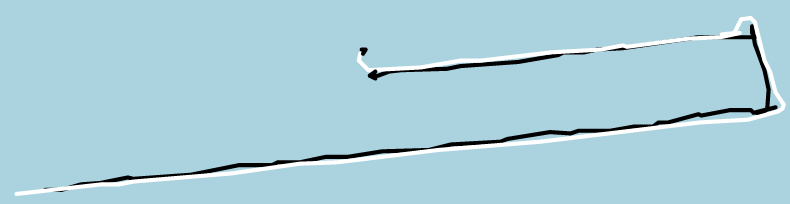
\includegraphics[width=0.8\textwidth]{figures/ScreenshotToResultsPNG2.png}}%
   \\
    \subfloat[Speed and Distance data]{\label{fig:setup2}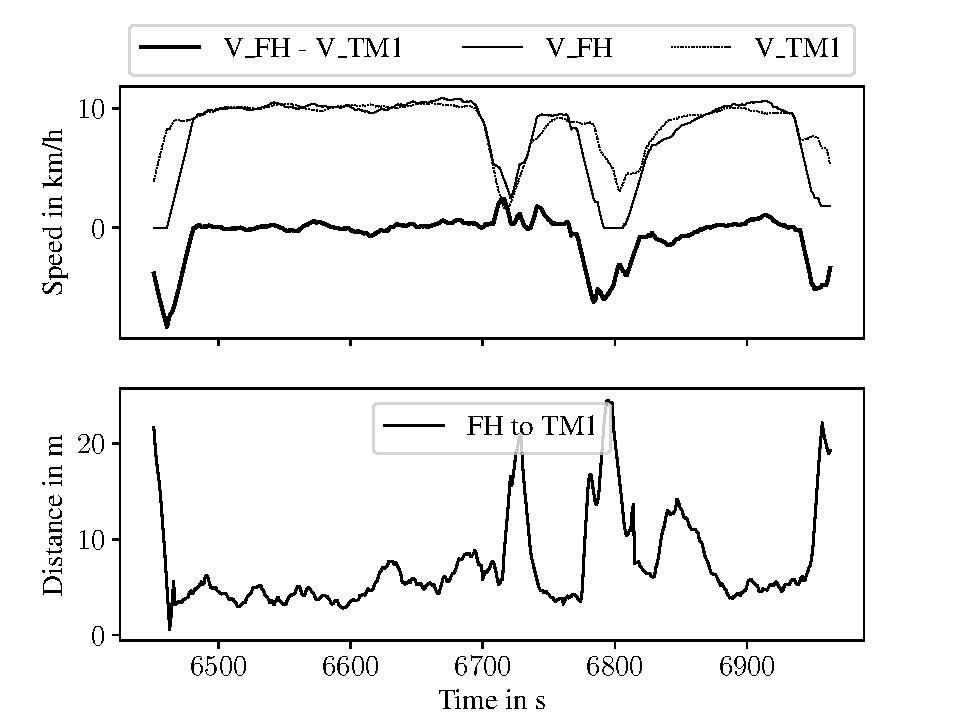
\includegraphics[width=0.9\textwidth]{figures/stacked_plotted_data_platoon}}
    \caption{A \ac{FH} and a \ac{TM} in harvest and overloading scenario, which is represented as distance and speed data plotted in regards to the
   time and which is visualised as a black and white travel lane for the \ac{FH}, \ac{TM} respectively}%
    \label{fig:setups12}%
\end{figure}

The data points of a detected harvest and overloading scenario are represented in \autoref{fig:setups12}.
The \ac{FH} and \ac{TM}, plotted as black and white lines respectively, drive from the left lower corner to the top middle of the map in \autoref{fig:setup1}.
In between, the \ac{FH} and \ac{TM} do \num{2} turning manoeuvres on the right side of the map in \autoref{fig:setup1}.
At the end of the scenario, the \ac{TM} turns to the right and heads towards the field exit.

The plotted distance and velocity data in \autoref{fig:setup2} illustrates the same events.
In the beginning, the \ac{TM} drives with a higher velocity to catch up with the \ac{FH}'s position.
After that, the \ac{TM} and \ac{FH} drive with a similar velocity and a distance below \SI{10}{\metre} down the field lane.
As soon as a turning manoeuvre starts, the distance increases and the velocity difference can be seen.
After every turning manoeuvre, the \ac{TM} and \ac{FH} drive again with a similar velocity and a distance below \SI{10}{\metre}.
In the end, when the \ac{TM} is full and leaves the harvest and overloading scenario, the distance increases and the \ac{TM} drives at a higher velocity.

\begin{figure}%
   \centering
   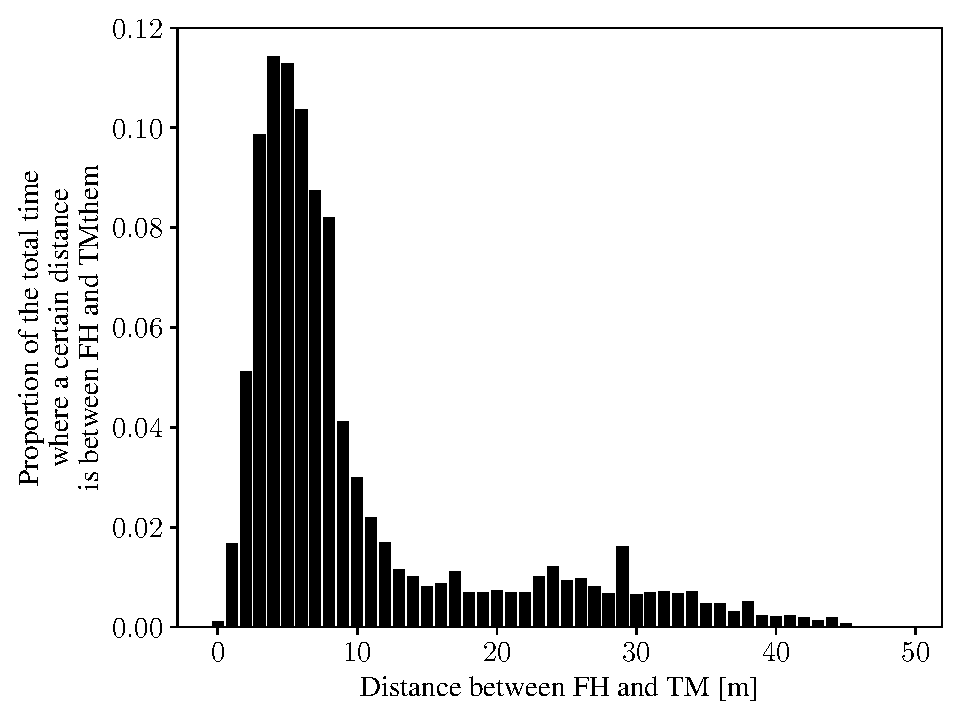
\includegraphics[width=0.85\textwidth]{figures/distanceHarvestScenario}
   \caption{Distribution of time proportions where a given distance was between \acf{FH} and \acf{TM} in a harvest platoon scenario.}%
   \label{fig:distance}%
\end{figure}
\begin{figure}%
   \centering
   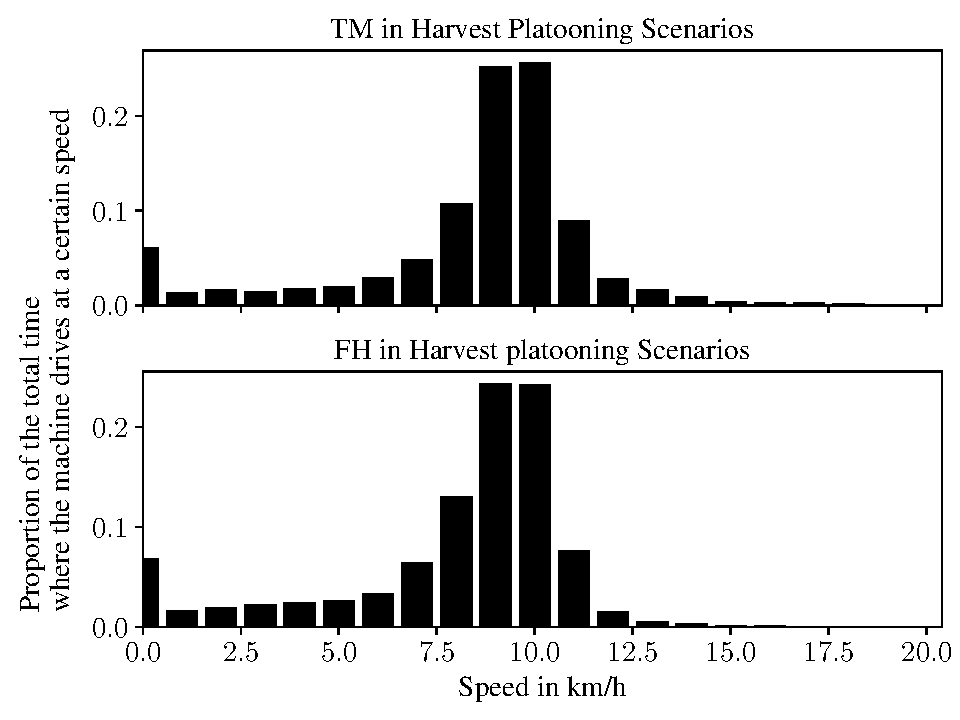
\includegraphics[width=0.85\textwidth]{figures/speedHarvestScenario}
   \caption{Distribution of time proportions where \acf{FH} and \acf{TM} drove with a certain speed in a harvest platoon scenario}%
   \label{fig:speed}%
\end{figure}
For the detected data points of the platooning services from recorded data of the corn harvest,
the proportion where the \ac{FH} and \ac{TM} move in a specific distance is shown in \autoref{fig:distance}.
For the same data points, the proportion in which \ac{FH} and \ac{TM} move at a given speed is available in \autoref{fig:speed}.

These analysing results show that the \ac{TM} and the \ac{FH} usually move with a distance of less than \SI{10}{\metre}.
In addition, the distance can also be higher, e.g. in turning manoeuvres or before the overloading process.

\textcite{smolnik_5g_2020} specifies the required communication range of platooning services in the corn harvest process
as less than \SI{30}{\metre}.

One notable observation in \autoref{fig:speed} is that the \ac{FH} and \ac{TM}s in the corn harvesting platooning scenario
often travel at a speed of approximately \SI{10}{\kilo\metre\per\hour}.
This speed is significantly higher than the average speed of \SIrange{6.6}{8.1}{\kilo\metre\per\hour} (\SIrange{1.9}{2.2}{\metre\per\second}) of a \ac{FH} operating on a \SI{80}{\hectare} field from \cite{faustzahlen2018}.
\textcite{nedelcu_influence_2020} report a optimal working speed of \SIrange{2.6}{6.3}{\kilo\metre\per\hour} (\SIrange{0.73}{1.75}{\metre\per\second}) for a \ac{FH} which depends on the \ac{PD}.


It is necessary to classify that in the year of the recorded data was little precipitation, so the corn was not dense and high,
and the last speed value is an average value of the entire corn harvest process,
which can be calculated from the data in \cite{faustzahlen2018}.
Nevertheless, the recorded data shows that a platooning service in agriculture must also be designed for higher speeds.

In \autoref{fig:speed} is a local maximum at a speed of \SI{0}{\kilo\metre\per\hour}.
In a harvest platoon scenario, \ac{FH} and \ac{TM} can stand still briefly when the cutting device is jammed.
The driver's specific actuation usually clears the forage jam of the cutting device so that the platoon can continue its work.

\textcite{smolnik_5g_2020} defines an average speed of \SI{4.5}{\kilo\metre\per\hour} for the development of platooning
services in the corn harvesting process.
Depending on the \ac{PD}, the speed can vary from \SIrange{2}{6}{\kilo\metre\per\hour} according to the authors.
The authors do not give a basis for the figures.
However, the report is from the agricultural machinery manufacturer Claas,
which is a major producer of \ac{FH} worldwide and thus can be regarded as having good knowledge of the topic.

\textcite{klingler_agriculture_2018} investigated the suitability of IEEE 802.11p for \ac{WIC}.
The authors detected that shadowing effects occur in the harvest scenario.
The authors explain the effect because another tractor or the spout of the \ac{FH} was in \ac{LOS}.
\begin{figure}%
   \centering
   \begin{tikzpicture}
      \node[label=below right:FH](a) at (0,0) {\textbullet};
      \node[label=above:North](d) at (0,1) {\textbullet};
      \node[label=above:Heading](c) at (1,1.5) {\textbullet};
      \node[label=below:TM](b) at (2,0) {\textbullet};
      \node[label=below:FH\_previous](e) at (-1,-1.5) {\textbullet};
      \node[label=above:North](f) at (-1,-0.5) {\textbullet};
      \draw [thick] (a) -- (b);
      \draw [thick] (a) -- (c);
      \draw [thick] (a) -- (d);
      \draw [thick] (a) -- (e);
      \draw [thick] (e) -- (f);
      \draw
      pic["$\beta$", draw, <-,angle eccentricity=0.8, angle radius=1.0cm]
      {angle=b--a--d}
      pic["$\alpha$", draw, <-,angle eccentricity=1.2, angle radius=1.0cm]
      {angle=a--e--f}
      pic["$Relative\ Bearing$", draw, <-, angle eccentricity=1.8, angle radius=1.5cm]
      {angle=b--a--c};
   \end{tikzpicture}
   \caption{Relative bearing between \ac{FH} and \ac{TM} which is calculated using the previous location of \ac{FH} by using $\beta$ and $\alpha$ for \autoref{eq:RelativeBearing}}%
   \label{fig:bearing_fh_tm}%
\end{figure}
I reviewed the recorded position data to get an overview of the \ac{TM}'s position relative to the \ac{FH} in the overloading process. The relative bearing is the angle between the position of the \ac{TM} and the heading of the position of the \ac{FH}. Using the previous position of the \ac{FH}, the relative bearing between \ac{FH} and \ac{TM} can be calculated with the angles $\alpha$ and $\beta$ in \autoref{fig:bearing_fh_tm} as:
\begin{equation}\label{eq:RelativeBearing}
   Relative\_Bearing = \beta - \alpha ,
\end{equation}
Assuming that the \ac{FH} does not move backwards, the relative bearing describes the relative angle from the
\ac{FH} to \ac{TM}.
The result is displayed in \autoref{fig:bearing}.
It can be observed that the \ac{TM} is mainly close to the \ac{FH} at an angle of \SIrange{30}{150}{\degree} at
a distance between \SIrange{0}{10}{\metre}.

\begin{figure}[H]
   \centering
   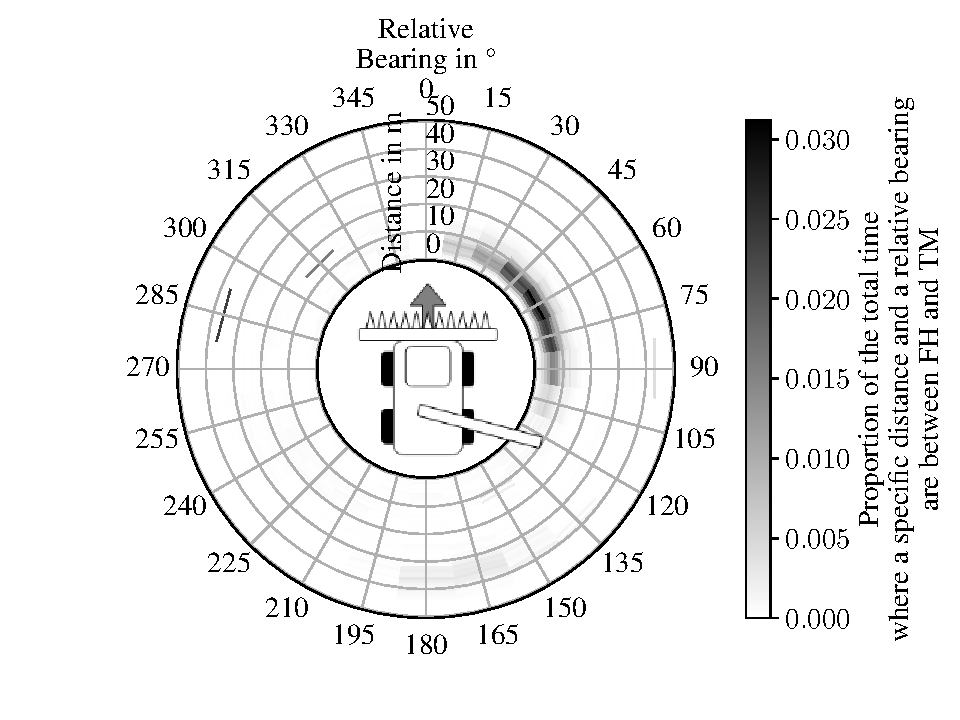
\includegraphics[width=0.99\textwidth]{figures/bearingHarvestScenario50.pdf}
   \caption{Distribution of time proportion at specific distances and relative bearings between \acf{FH} and \acf{TM}}%
   \label{fig:bearing}%
\end{figure}

In addition, it is noticeable that the machine can also be directly behind the \ac{FH}.
This driving behind each other is typical when a new part of the field is being cut in harvesting,
as shown in \autoref{fig:startpart}.
When there is a greater distance between \ac{TM} and \ac{FH}, the \ac{TM} is usually behind the FH at an angle of
\SIrange{157.5}{187.5}{\degree}.
At these moments, the \ac{TM} is empty and closes up to the \ac{FH} to operate in a new platooning Service together.

\begin{figure}[H]%
   \centering
   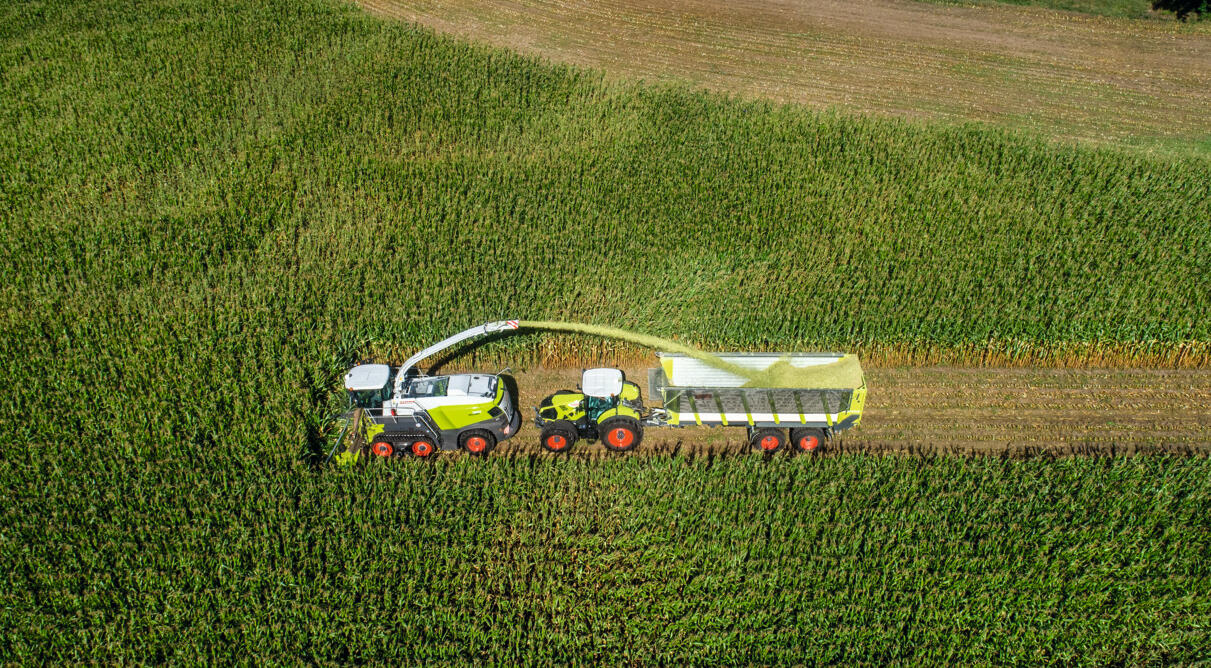
\includegraphics[width=0.8\textwidth]{figures/claas_harvest_behind.png}
   \caption{\acf{FH} and \acf{TM} start cutting a new field section}%
   \label{fig:startpart}%
\end{figure}

Another notable fact is that the \ac{TM} hardly ever stayed to the left of the \ac{FH}.
Since the \ac{FH} often made left turns, the crop was usually already harvested to the right of the \ac{FH} so
that the \ac{TM} could drive there without running over the crop.
On rare occasions, the \ac{TM} was also to the left of the \ac{FH}.
Such a platooning scenario can be an exception or a driving manoeuvre to start cutting a new part of the field.

The results reveal only a first impression of the requirements of the harvest and loading process.
More data from around the world must be analysed to make a general statement.
The low rainfall this year has already resulted in a low plant population.
This field condition made a higher process speed possible.
The data may also vary on the size of the agricultural machinery.
Using a smaller \ac{FH} would result in a smaller distance between \ac{TM} and \ac{FH}.
To make a general statement, I should use data from different years, machines or harvest and loading scenarios
because they can reveal other initial field conditions.
git

\begin{comment}
	\TODO{
	Heading Annahme Vorwärts Fahrt. Ansonsten Überprüfen und nochmal Einzelfahrt plotten und anschauen.
	Wie oft dreht sich das Heading ?
	Möglicherweise Rückwärtsfahrt erkennen? Oder WIC Requirements erwähnen? }
\end{comment}

